\medskip

\textbf{Partie 1}

Puisque la commande est faite au hasard, on assimile les proportions à des probabilités. On en déduit l'arbre pondéré suivant :

	
	\begin{center}
	
	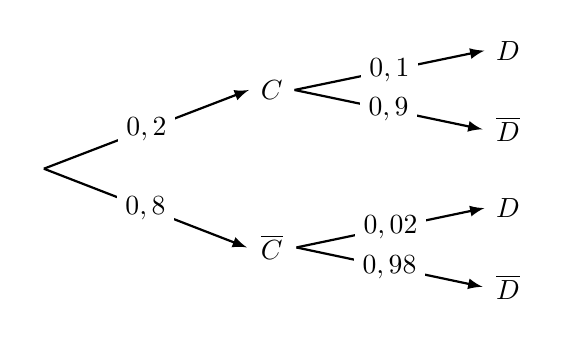
\begin{tikzpicture}[xscale=1,yscale=1]
	
	\tikzstyle{fleche}=[->,>=latex,thick]
	\tikzstyle{noeud}=[fill=white,circle,inner sep=2pt]
	\tikzstyle{feuille}=[fill=white,circle,inner sep=2pt]
	\tikzstyle{etiquette}=[midway,fill=white, inner xsep=3pt, inner ysep=1.5pt]
	
	\def\DistanceInterNiveaux{3}
	\def\DistanceInterFeuilles{1}
	
	\def\NiveauA{(0)*\DistanceInterNiveaux}
	\def\NiveauB{(1)*\DistanceInterNiveaux}
	\def\NiveauC{(2)*\DistanceInterNiveaux}
	\def\InterFeuilles{(-1)*\DistanceInterFeuilles}
	
	\node[noeud] (R) at ({\NiveauA},{(1.5)*\InterFeuilles}) {$$};
	\node[noeud] (Ra) at ({\NiveauB},{(0.5)*\InterFeuilles}) {$C$};
	\node[feuille] (Raa) at ({\NiveauC},{(0)*\InterFeuilles}) {$D$};
	\node[feuille] (Rab) at ({\NiveauC},{(1)*\InterFeuilles}) {$\overline{D}$};
	\node[noeud] (Rb) at ({\NiveauB},{(2.5)*\InterFeuilles}) {$\overline{C}$};
	\node[feuille] (Rba) at ({\NiveauC},{(2)*\InterFeuilles}) {$D$};
	\node[feuille] (Rbb) at ({\NiveauC},{(3)*\InterFeuilles}) {$\overline{D}$};
		
		\draw[fleche] (R.east)--(Ra.west) node[etiquette] {$0,2$};
		\draw[fleche] (Ra.east)--(Raa.west) node[etiquette] {$0,1$};
		\draw[fleche] (Ra.east)--(Rab.west) node[etiquette] {$0,9$};
		\draw[fleche] (R.east)--(Rb.west) node[etiquette] {$0,8$};
		\draw[fleche] (Rb.east)--(Rba.west) node[etiquette] {$0,02$};
		\draw[fleche] (Rb.east)--(Rbb.west) node[etiquette] {$0,98$};
	\end{tikzpicture}
	\end{center}
	

\begin{enumerate}
\item 	$\mathrm{P}(C\cap D) = \mathrm{P}(C) \times \mathrm{P}_C(D) = 0,2 \times 0,1 = 0,02$.

La probabilité d'avoir un casque contrefait présentant un défaut est donc de 0,02.

\item Les évènements $C$ et $\overline{C}$ forment une partition de l'univers, donc, d'après la loi des probabilités totales, on en déduit :

$\begin{aligned}[t] \mathrm{P}(D) &= \mathrm{P}(C \cap D) + \mathrm{P}\left(\overline{C} \cap D\right)\\
&= 0,02 + 0,8 \times 0,02\\
&= 1,8 \times 0,02\\
&= 0,036\end{aligned}$

La probabilité de commander un casque présentant un défaut de conception est donc de 0,036.
\item On demande ici de calculer la probabilité conditionnelle : $\mathrm{P}_D(C)$

$\mathrm{P}_D(C) = \dfrac{\mathrm{P}(C \cap D)}{\mathrm{P}(D)} = \dfrac{0,02}{0,036} = \dfrac{5}{9} \approx 0,556$ à $10^{-3}$ près.
\end{enumerate}

\medskip

\textbf{Partie 2}
\begin{enumerate}
\item 
	\begin{enumerate}
		\item 
		
\begin{itemize}
\item On a une expérience aléatoire de base (on commande un casque), pour laquelle on considère deux issues. Pour cette épreuve de Bernoulli, le succès (le casque présente un défaut) a une probabilité $p = 0,036$. (d'après la question \textbf{2.} de la \textbf{partie 1});
\item On répète cette expérience $n=35$ fois, de façon indépendante (puisque la répétition est assimilable à un tirage \textbf{avec} remise);
\item La variable aléatoire $X$ compte le nombre de succès sur les 35 répétitions.
\end{itemize}

Ces éléments permettent de confirmer que $X$ suit la loi binomiale $ \mathcal{B}(35~;~0,036) $

\item On veut calculer $\mathrm{P}(X = 1)$.

$ \mathrm{P}(X = 1) = \displaystyle \binom{35}{1} \times 0,036^1 \times (1 - 0,036)^{35- 1} = 35 \times 0,036 \times 0,964^{34} \approx 0,362 $ à $ 10^{-3} $ près.

\item Calculons : $\mathrm{P}(X \leqslant 1) = \mathrm{P}(X = 0) + \mathrm{P}(X = 1) \approx 0,639$ à $ 10^{-3} $ près (à la calculatrice).
	\end{enumerate}

	\item Ici, pour tout entier $n$ naturel non nul, on peut créer une variable aléatoire $X_n$ qui suit la loi binomiale $ \mathcal{B}(n~;~0,036) $.

	Pour $n$ un entier naturel non nul, la probabilité qu'un casque au moins présente un défaut sur $n$ casques commandés est donc :

$\mathrm{P}(X_n \geqslant 1) = 1 - \mathrm{P} (X_n = 0) = 1 - \displaystyle \binom{n}{0}\times 0,036^0 \times 0,964^{n} = 1 - 0,964^{n}$.

On résout donc sur $\N^*$ :

$\begin{aligned}[t] \mathrm{P}(X_n \geqslant 1) \geqslant 0,99
&\iff 1 - 0,964^{n} \geqslant 0,99\\
&\iff -0,964^n \geqslant -0,01\\
&\iff 0,964^n \leqslant 0,01\\
&\iff \ln(0,964^n) \leqslant \ln(0,01) \quad \text{car ln est croissante sur }\R^{*+} \\
&\iff n\ln(0,964) \leqslant \ln(0,01)\\
&\iff n \geqslant \dfrac{\ln(0,01)}{\ln(0,964)} \qquad \text{car} \ln(0,964) <0
\end{aligned}$

or $\dfrac{\ln(0,01)}{\ln(0,964)}\approx 125,6$, donc les solutions sont les entiers naturels supérieurs ou égaux à 126.

Il faut donc commander au moins 126 casques pour que la probabilité d'en avoir au moins un défectueux soit supérieure à 0,99.

\end{enumerate}

\bigskip
